\chapter{Líneas futuras}\label{cap:7}
\lettrine{L}{as posibles perspectivas de futuro} relacionadas con esta línea de trabajo ofrecen distintos caminos, cada uno de los cuales podrían constituir nuevos Trabajos Fin de Grado o Fin de Máster. A partir de los resultados presentados durante el capítulo \S\ref{cap:4}, resumidas en el capítulo \S\ref{cap:5}, existen varias alternativas y combinaciones a explorar para intentar comprender o solucionar algunas de las incógnitas pendientes de resolver completamente: distribución radial de fase y adición del momento angular orbital.

En primer lugar, aunque el acuerdo obtenido entre experimento y simulaciones del perfil radial de intensidad es adecuado, esto sucede debido a que una parte importante de las modificaciones y esfuerzos han sido dedicados a conseguir reproducir la forma de la curva con la mayor precisión posible, mientras que el perfil de fase de los fotones han quedado relegados a un segundo plano, prestando atención simplemente a la formación de la pareja de picos y el valle, simétricamente centrados en la columna de plasma. Sin embargo, la profundidad entre los picos y valle de fase de las simulaciones necesita aproximarse mejor a las observaciones, intentando mantener la distribución de intensidad radial conseguida.

Esta pequeña discrepancia, relativa a la fase de la amplificación ultravioleta extrema (\acrshort{xuv}) obtenida, está relacionada con la introducción de la columna de plasma inicial para el guiado de la semilla de armónicos de alto orden (\acrshort{hoh}) y los pulsos láser en el infrarrojo cercano (\acrshort{nir}). La expansión hidrodinámica del plasma origina un índice de refracción decreciente en dirección radial, esto es, un gradiente de densidad electrónica radial creciente que, en última instancia, es responsable de la distribución de fase de los fotones. Por tanto, futuros trabajos podrían dirigir sus esfuerzos en realizar nuevos cambios del perfil radial de densidad electrónica, utilizando una metodología similar a la empleada para reducir la diferencia entre los máximos y mínimos locales del laboratorio y de las simulaciones.

En segundo lugar, la adición del momento angular orbital (\acrshort{oam}) constituye probablemente el aspecto más interesante a la hora de continuar en futuros trabajos. En general, los resultados obtenidos en combinación con la función exponencial a trozos, introducida para definir la región del canal con \ce{Kr^{8+}}, necesitarán explicarse satisfactoriamente por nuevos estudios. Además, este objetivo podría conseguirse y ampliarse recurriendo, o bien a la introducción del \acrshort{oam} en secciones estudiadas durante el proyecto como, por ejemplo, las sigmoides, o bien mediante otras funciones (recurriendo tal vez a polinomios interpoladores) que puedan reconstruir la frontera de iones \ce{Kr^{8+}} en el plasma.

De este modo, y en línea con el primer punto comentado, también cabría la posibilidad de terminar agrupando estos resultados de intensidad, fase y \acrshort{oam} en un solo sistema de simulación láser-plasma, intentando optimizar otros parámetros como la intensidad máxima del pulso láser infrarrojo \acrshort{nir} a la entrada del columna, la duración de los pulsos participantes, o las características de la semilla \acrshort{hoh} inyectada, tanto intrínsecas como relativas a los demás haces láser, por ejemplo los tiempos de retardo. Así, el objetivo consistiría en mejorar la eficiencia de la conversión de energía ---y la deposición de energía--- tanto del láser \acrshort{nir} de bombeo como durante la amplificación \acrshort{xuv} de la semilla \acrshort{hoh}, que podrían ayudar a capturar de manera más precisa la complejidad de estos sistemas multiescala.

\begin{figure}[htbp]
  \centering
  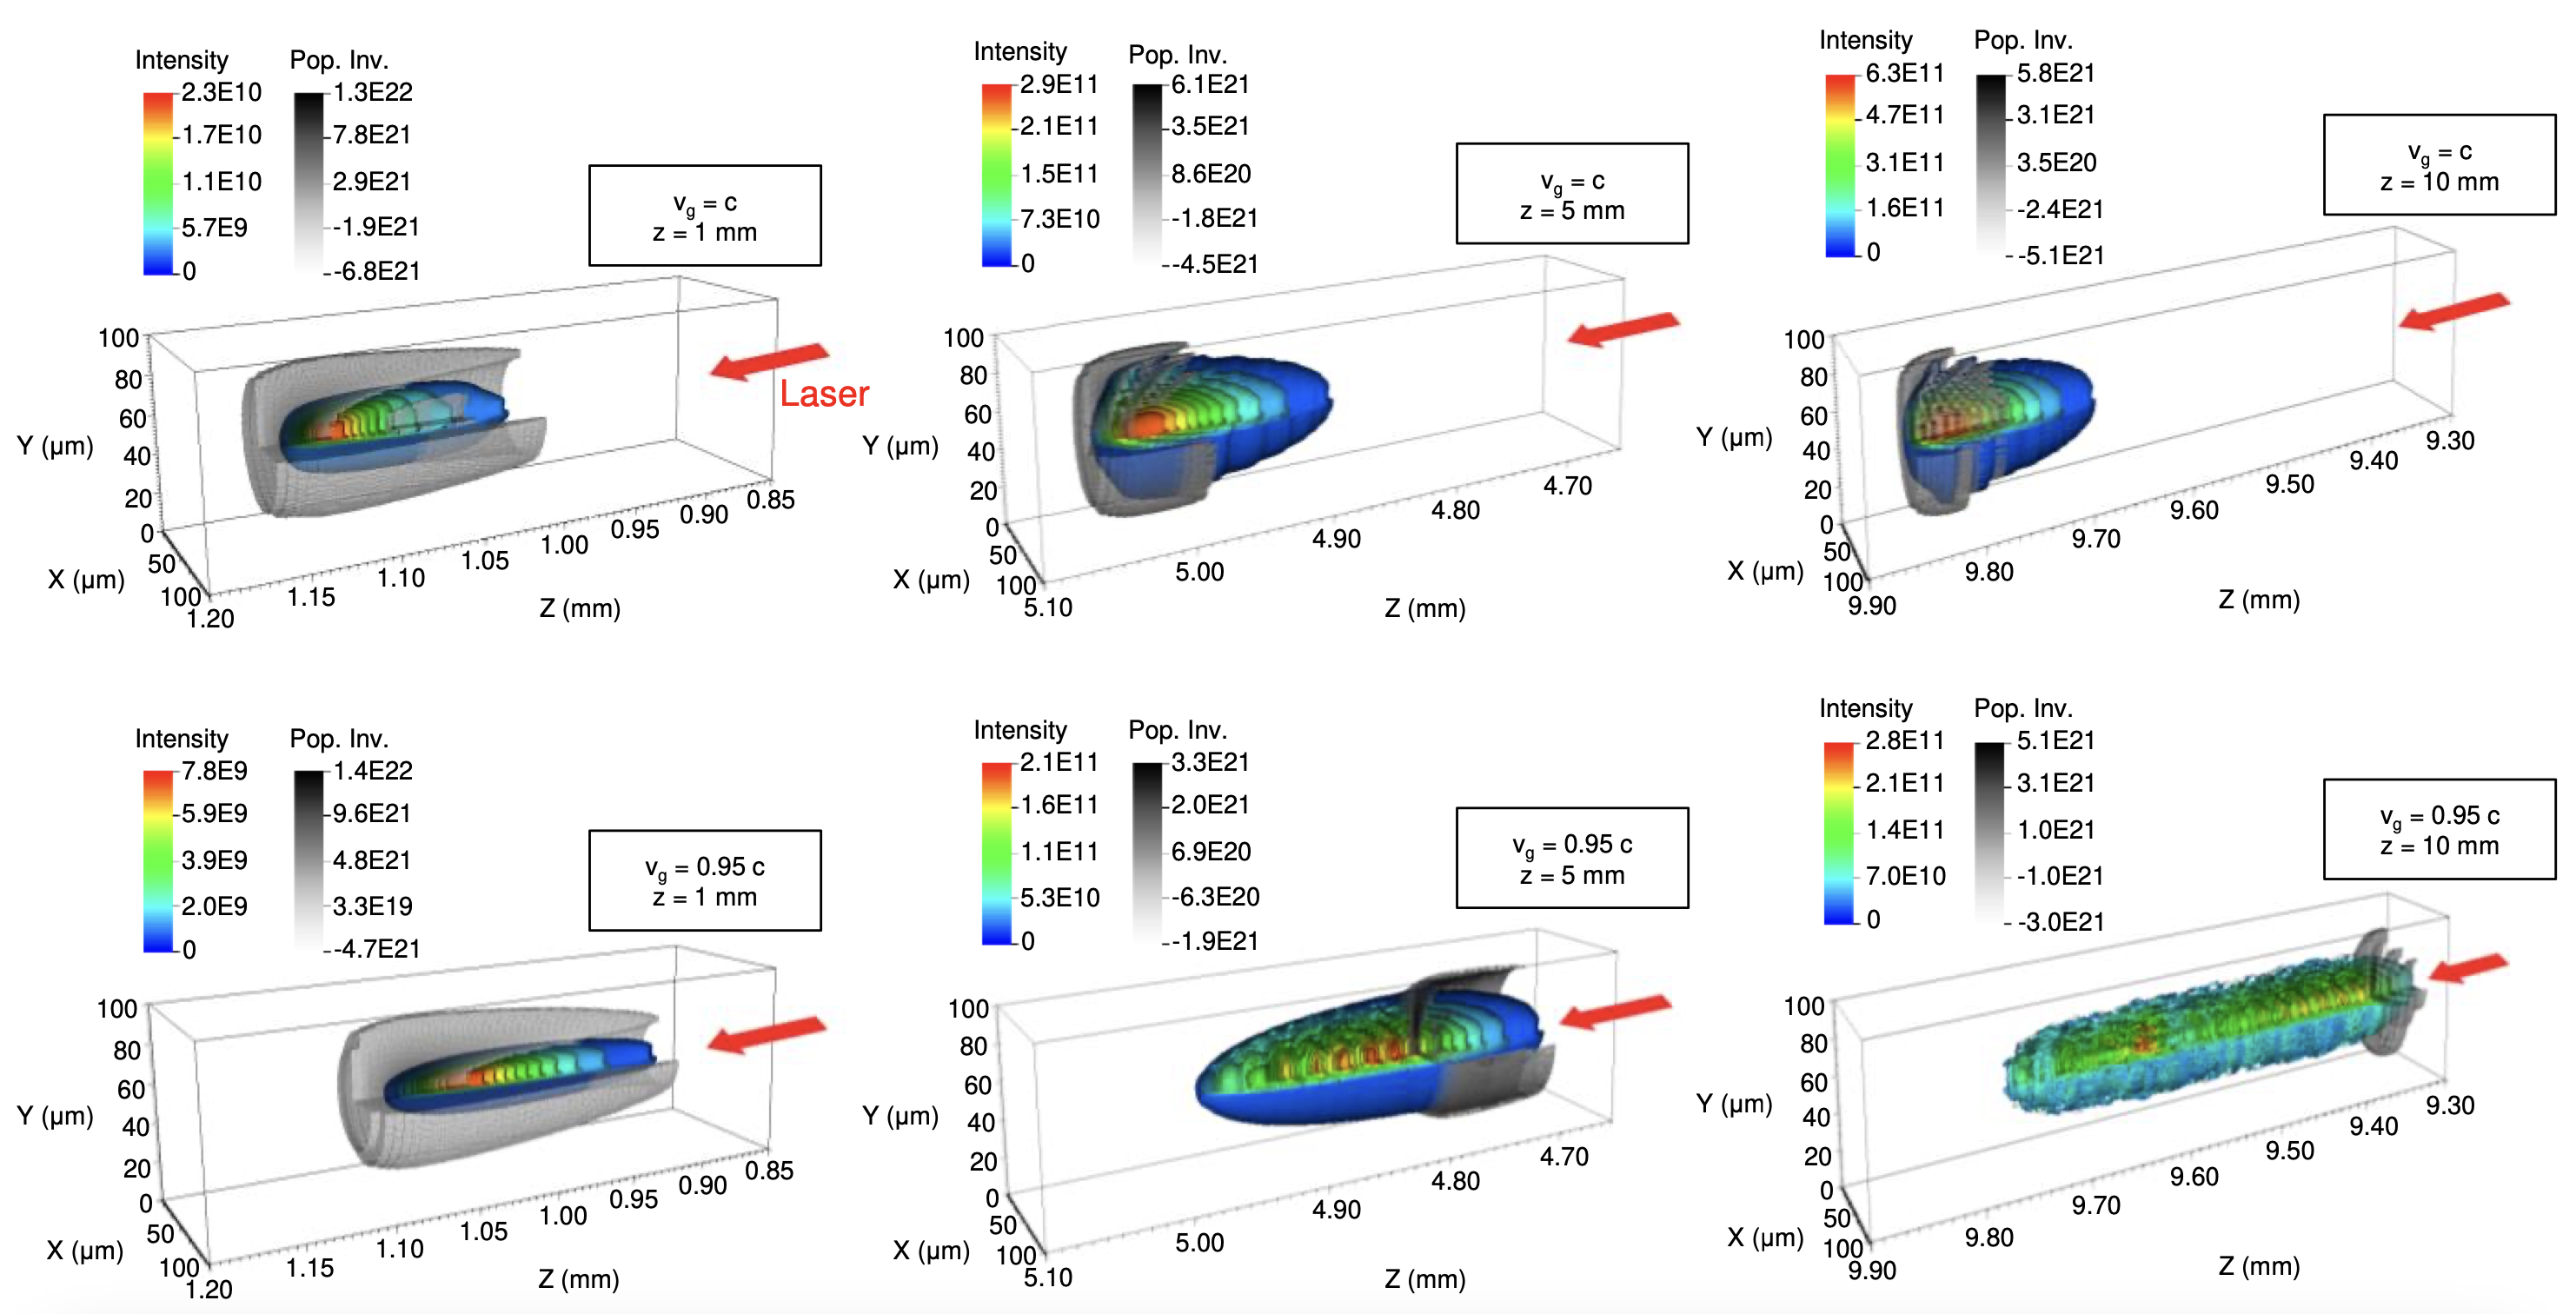
\includegraphics[width=0.8\textwidth]{Figuras/ch7_futuro.png}
  \caption{Simulaciones en tres dimensiones\autocite{Kabacinski2023} con Dagon de la amplificación \acrshort{sxrl} para dos velocidades de grupos distintas, a distintas longitudes de propagación}
  \label{fig:7.1}
\end{figure}

Por último, otra buena región de exploración en posteriores estudios podría incluir la velocidad de propagación de la onda a través del plasma. Aunque no ha sido mencionado anteriormente, existe una desincronización natural entre la semilla \acrshort{hoh} y el pulso \acrshort{nir} de bombeo, producido por las diferentes velocidades de grupo en el interior del plasma. A menor frecuencia, menor velocidad (dispersión negativa), provocando un desacoplamiento entre la semilla \acrshort{hoh} ---que viaja más rápido--- y el haz infrarrojo ---que viaja más lento---, repercutiendo negativamente a la ventana de ganancia. 

Un estudio reciente\autocite{Kabacinski2023} ha demostrado la posibilidad de mejorar la eficiencia de la extracción de energía controlando esta velocidad de grupo, utilizando la secuencia de códigos de este trabajo para simular numéricamente el procedimiento experimental propuesto. El código Dagon incorpora la velocidad de grupo como un parámetro más que puede variarse a voluntad (como muestra la Figura \S\ref{fig:7.1}), permitiendo añadir un grado de libertad adicional a través de la velocidad de la onda, optimizando el fenómeno de la amplificación.

En definitiva, continuar este ámbito de investigación en particular contribuirá a esclarecer su posible interés en investigación, así como en las aplicaciones de formación de imágenes y diagnosis, o en conseguir fuentes de radiación \acrshort{xuv} coherente más pequeñas y eficientes. 
